% begin module cardioid-ex7
\begin{frame}
\begin{example} %[Example 7, p. 679]
Sketch the curve $r = 1 + \sin \theta$.
\begin{columns}[c]
\column{.3\textwidth}
\psset{xunit=1cm, yunit=1cm}
\begin{pspicture}(-1.499038, -0.700000)(1.6,2.4) 

\tiny 
\psaxesStandard{-1.4}{-0.6}{1.4}{2.3}
\psLabelXOne
\psLabelYOne
\uncover<2-6>{
%Calculator input: plotCurve{}(\cos{}t \sin{}t+\cos{}t, \sin^{2}{}t+\sin{}t, 0, 2 \pi)
\parametricplot[arrows=->, linecolor=\psColorGraph, plotpoints=200] {0}{0.7}{t 57.29578 mul cos t 57.29578 mul sin t 57.29578 mul cos mul add t 57.29578 mul sin t 57.29578 mul sin 2.0000000 exp add }
%Calculator input: plotCurve{}(\cos{}t \sin{}t+\cos{}t, \sin^{2}{}t+\sin{}t, 0, 2 \pi)
\parametricplot[linecolor=\psColorGraph, plotpoints=200] {0.7}{1.570796327} {t 57.29578 mul cos t 57.29578 mul sin t 57.29578 mul cos mul add t 57.29578 mul sin t 57.29578 mul sin 2.0000000 exp add }
}
%\uncover<3-6>{%
%\psFullDot{1.207107}{1.207107}
%}
\uncover<handout:0| 3>{%
\psline[linecolor=blue](0,0)(1.207107, 1.207107)
\psAngle{0}{0.785398}{0.4}{$\theta$}
\rput[b](0.6, 0.68){$r$}
} 
%\uncover<4-6>{%
%\psFullDot{1.017510}{1.522811}
%}
\uncover<handout:0| 4>{%
\psline[linecolor=blue](0,0)(1.017510, 1.522811)
\psAngle{0}{0.981748}{0.4}{$\theta$}
\rput[b](0.45, 0.8){$r$}
}
%\uncover<5-6>{%
%\psFullDot{0.736237}{1.777433}
%}
\uncover<handout:0| 5>{
\psline[linecolor=blue](0,0)(0.736237, 1.777433)
\psAngle{0}{1.178097}{0.4}{$\theta$}
\rput[b](0.3, 0.9){$r$}
}
%\uncover<6>{%
%\psFullDot{0.386432}{1.942725}
%} 
\uncover<handout:0| 6>{
\psAngle{0}{1.374447}{0.4}{$\theta$}
\psline[linecolor=blue](0,0)(0.386432, 1.942725)
\rput[b](0.1, 1.1){$r$}
} 
\uncover<handout:0| 7->{
%Calculator input: plotCurve{}(\cos{}t \sin{}t+\cos{}t, \sin^{2}{}t+\sin{}t, 0, 2 \pi)
\parametricplot[plotpoints=400, linecolor=blue] {0}{1.570796327}{t 57.29578 mul cos t 57.29578 mul sin t 57.29578 mul cos mul add t 57.29578 mul sin t 57.29578 mul sin 2.0000000 exp add }
}

\uncover<7>{
%Calculator input: plotCurve{}(\cos{}t \sin{}t+\cos{}t, \sin^{2}{}t+\sin{}t, 0, 2 \pi)
\parametricplot[arrows=->, linecolor=\psColorGraph, plotpoints=200] {1.570796327}{2.35619449}{t 57.29578 mul cos t 57.29578 mul sin t 57.29578 mul cos mul add t 57.29578 mul sin t 57.29578 mul sin 2.0000000 exp add }
%Calculator input: plotCurve{}(\cos{}t \sin{}t+\cos{}t, \sin^{2}{}t+\sin{}t, 0, 2 \pi)
\parametricplot[linecolor=\psColorGraph, plotpoints=200] {2.35619449}{3.141592654} {t 57.29578 mul cos t 57.29578 mul sin t 57.29578 mul cos mul add t 57.29578 mul sin t 57.29578 mul sin 2.0000000 exp add }
}
\uncover<handout:0| 8->{
%Calculator input: plotCurve{}(\cos{}t \sin{}t+\cos{}t, \sin^{2}{}t+\sin{}t, 0, 2 \pi)
\parametricplot[linecolor=blue, plotpoints=200] {1.570796327}{3.141592654} {t 57.29578 mul cos t 57.29578 mul sin t 57.29578 mul cos mul add t 57.29578 mul sin t 57.29578 mul sin 2.0000000 exp add }
}
\uncover<8>{
%Calculator input: plotCurve{}(\cos{}t \sin{}t+\cos{}t, \sin^{2}{}t+\sin{}t, 0, 2 \pi)
\parametricplot[arrows=->, linecolor=\psColorGraph, plotpoints=200] {3.141592654}{3.926990817}{t 57.29578 mul cos t 57.29578 mul sin t 57.29578 mul cos mul add t 57.29578 mul sin t 57.29578 mul sin 2.0000000 exp add }
%Calculator input: plotCurve{}(\cos{}t \sin{}t+\cos{}t, \sin^{2}{}t+\sin{}t, 0, 2 \pi)
\parametricplot[linecolor=\psColorGraph, plotpoints=200] {3.926990817}{4.71238898} {t 57.29578 mul cos t 57.29578 mul sin t 57.29578 mul cos mul add t 57.29578 mul sin t 57.29578 mul sin 2.0000000 exp add }
}
\uncover<handout:0| 9->{
%Calculator input: plotCurve{}(\cos{}t \sin{}t+\cos{}t, \sin^{2}{}t+\sin{}t, 0, 2 \pi)
\parametricplot[linecolor=blue, plotpoints=200] {3.141592654}{4.71238898} {t 57.29578 mul cos t 57.29578 mul sin t 57.29578 mul cos mul add t 57.29578 mul sin t 57.29578 mul sin 2.0000000 exp add }
}
\uncover<9>{
%Calculator input: plotCurve{}(\cos{}t \sin{}t+\cos{}t, \sin^{2}{}t+\sin{}t, 0, 2 \pi)
\parametricplot[arrows=->, linecolor=\psColorGraph, plotpoints=200] {4.71238898}{5.7}{t 57.29578 mul cos t 57.29578 mul sin t 57.29578 mul cos mul add t 57.29578 mul sin t 57.29578 mul sin 2.0000000 exp add }
%Calculator input: plotCurve{}(\cos{}t \sin{}t+\cos{}t, \sin^{2}{}t+\sin{}t, 0, 2 \pi)
\parametricplot[linecolor=\psColorGraph, plotpoints=200] {5.7}{6.283185307} {t 57.29578 mul cos t 57.29578 mul sin t 57.29578 mul cos mul add t 57.29578 mul sin t 57.29578 mul sin 2.0000000 exp add }
}
\uncover<handout:0| 10->{
%Calculator input: plotCurve{}(\cos{}t \sin{}t+\cos{}t, \sin^{2}{}t+\sin{}t, 0, 2 \pi)
\parametricplot[linecolor=blue, plotpoints=200] {4.71238898}{6.283185307} {t 57.29578 mul cos t 57.29578 mul sin t 57.29578 mul cos mul add t 57.29578 mul sin t 57.29578 mul sin 2.0000000 exp add }
}

\end{pspicture} 

%\ \only<handout:0| 1>{%
%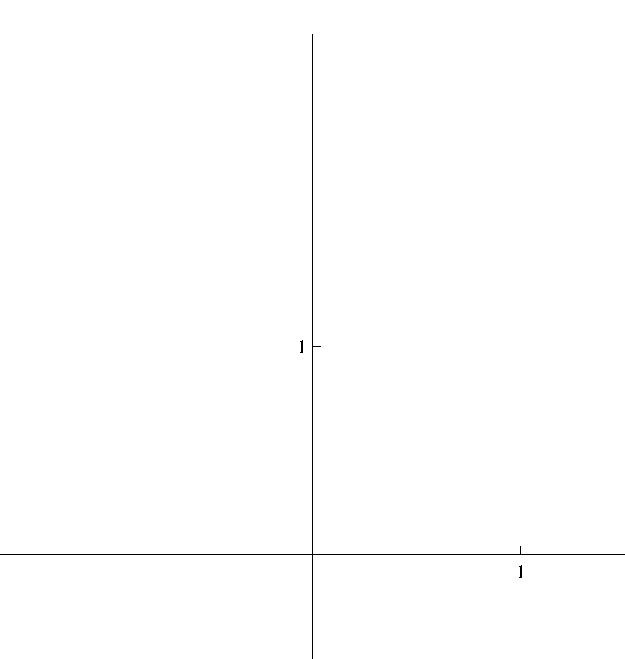
\includegraphics[height=3.6cm]{polar-curves/pictures/11-03-ex7a.pdf}%
%}%
%\only<handout:0| 2>{%
%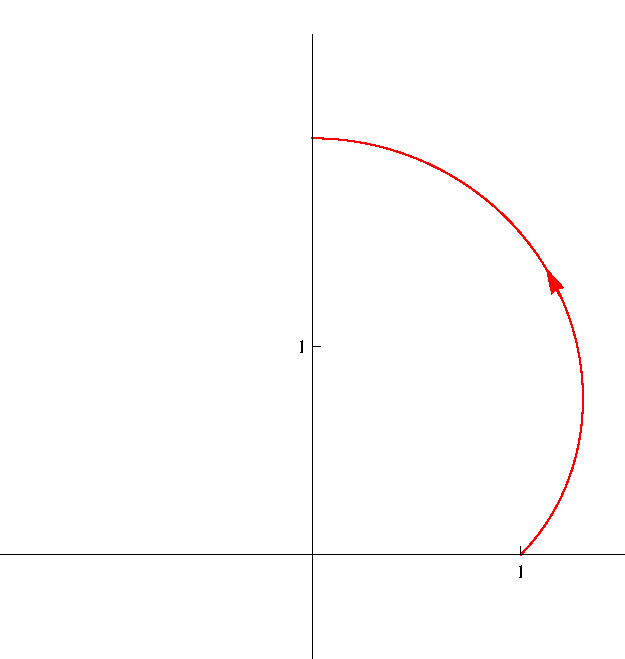
\includegraphics[height=3.6cm]{polar-curves/pictures/11-03-ex7b.pdf}%
%}%
%\only<handout:0| 3>{%
%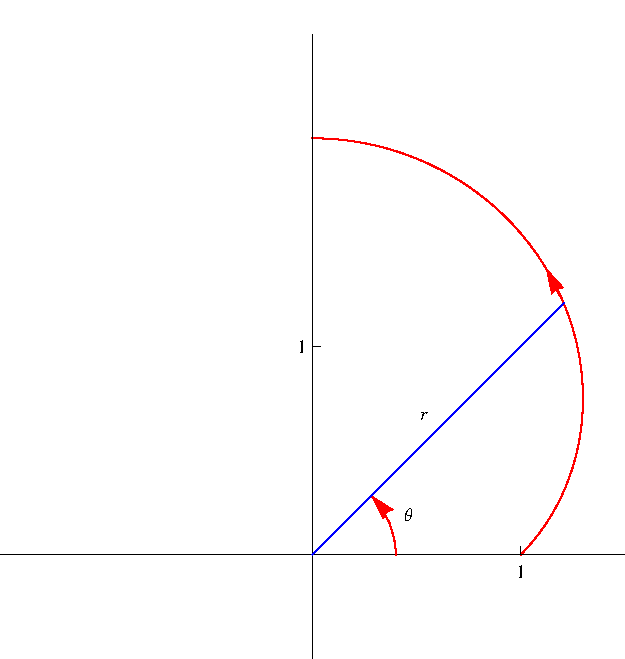
\includegraphics[height=3.6cm]{polar-curves/pictures/11-03-ex7ba.pdf}%
%}%
%\only<handout:0| 4>{%
%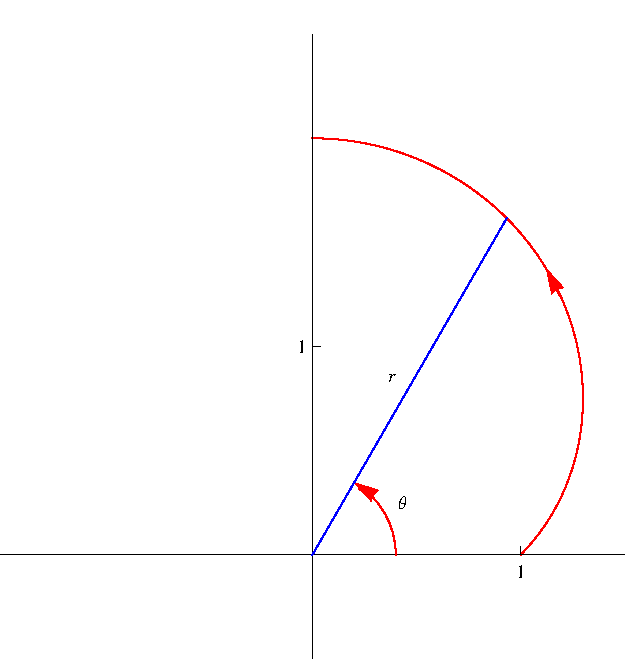
\includegraphics[height=3.6cm]{polar-curves/pictures/11-03-ex7bb.pdf}%
%}%
%\only<handout:0| 5>{%
%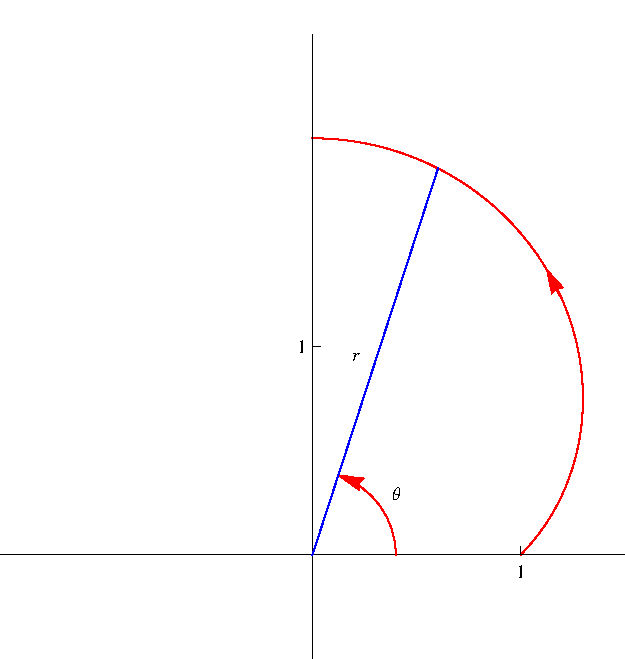
\includegraphics[height=3.6cm]{polar-curves/pictures/11-03-ex7bc.pdf}%
%}%
%\only<handout:0| 6>{%
%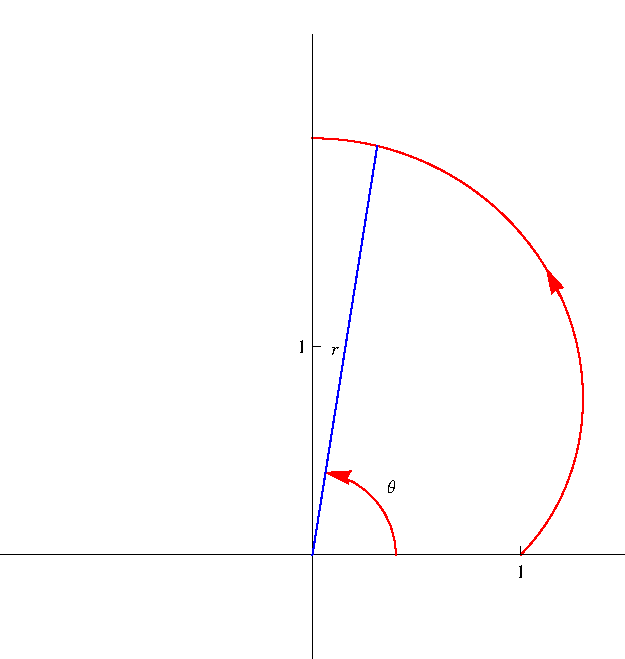
\includegraphics[height=3.6cm]{polar-curves/pictures/11-03-ex7bd.pdf}%
%}%
%\only<handout:0| 7>{%
%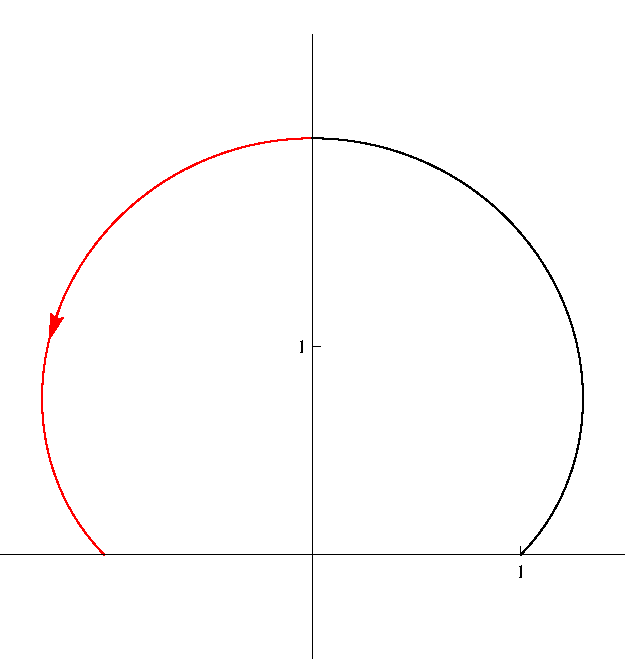
\includegraphics[height=3.6cm]{polar-curves/pictures/11-03-ex7c.pdf}%
%}%
%\only<handout:0| 8>{%
%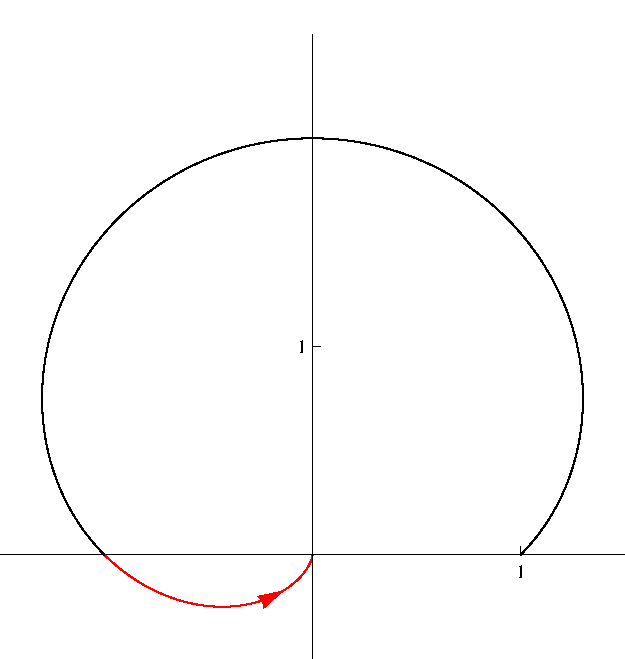
\includegraphics[height=3.6cm]{polar-curves/pictures/11-03-ex7d.pdf}%
%}%
%\only<9->{%
%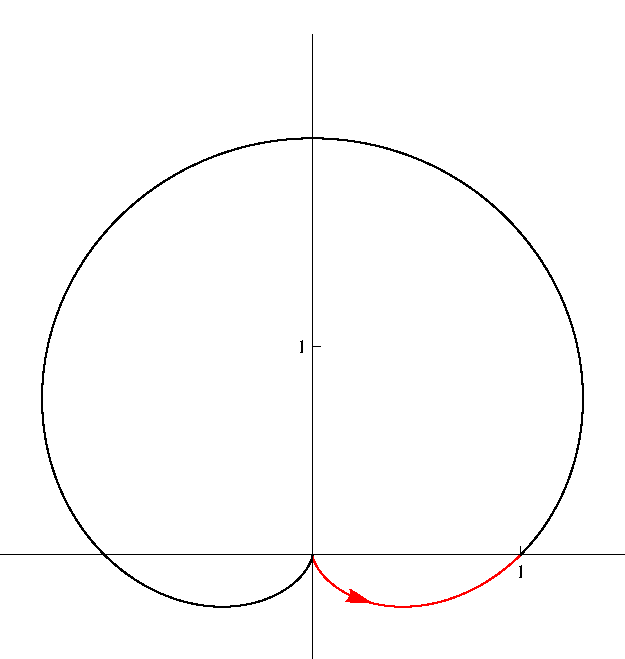
\includegraphics[height=3.6cm]{polar-curves/pictures/11-03-ex7e.pdf}%
%}%
\column{.7\textwidth}
\psset{xunit=1cm, yunit=1cm}
\begin{pspicture}(-0.700000, -0.700000)(6.55,2.4) 

\tiny 
\psframe*[linecolor=white](-0.7, -0.7)(6.55, 2.4)
\psaxes[arrows=<->, Dx=1.570796327, Dy=1, labels=none](0,0)(-0.5, -0.5)(6.4, 2.3)
\rput[r](-0.1,2.3){$r$}
\rput[t](6.48,-0.01){$\theta$}
\rput[r](-0.15,1){$1$}
\rput[r](-0.15,2){$2$}

\rput[t](! 1.570796327 -0.15){$\frac{\pi}2$}
\rput[t](! 1.570796327 2 mul -0.15){$\pi$}
\rput[t](! 1.570796327 3 mul -0.15){$\frac{3\pi}{2}$}
\rput[t](! 1.570796327 4 mul -0.15){$2\pi$}

\rput[l](3.4, 1){$r=1+\sin \theta$}

\uncover<handout:0| 3>{
\psLengthIndicator{0}{-0.1}{0.785398163}{-0.1}{$\theta$}
\psline[linecolor=blue](0.785398163, 0)(0.785398163, 1.707107)
}
\uncover<handout:0| 4>{
\psLengthIndicator{0}{-0.1}{0.981747704}{-0.1}{$\theta$}
\psline[linecolor=blue](0.981747704, 0)(0.981747704, 1.831470)
}
\uncover<handout:0| 5>{
\psLengthIndicator{0}{-0.1}{1.178097245}{-0.1}{$\theta$}
\psline[linecolor=blue](1.178097245, 0)(1.178097245, 1.923880)
}
\uncover<handout:0| 6>{
\psLengthIndicator{0}{-0.1}{1.374446786}{-0.1}{$\theta$}
\psline[linecolor=blue](1.374446786, 0)(1.374446786, 1.980785)
}


%Function formula: \sin{}x+1 
\psplot[linecolor=blue, plotpoints=1000]{0.000000}{6.283185}{1.0000000 x 57.29578 mul sin add }
\uncover<handout:0| 2-6>{
\psplot[linecolor=red, plotpoints=400]{0.000000}{1.570796327}{1.0000000 x 57.29578 mul sin add }
\psFullDot{0}{1}
\psFullDot{1.570796327}{2}
}
\uncover<handout:0| 7>{
\psplot[linecolor=red, plotpoints=400]{1.570796327}{3.141592654} {1.0000000 x 57.29578 mul sin add }
\psFullDot{1.570796327}{2}
\psFullDot{3.141592654}{1}
}
\uncover<handout:0| 8>{
\psplot[linecolor=red, plotpoints=400]{3.141592654} {4.71238898} {1.0000000 x 57.29578 mul sin add }
\psFullDot{3.141592654}{1}
\psFullDot{4.71238898}{0}
}
\uncover<handout:0| 9>{
\psplot[linecolor=red, plotpoints=400]{4.71238898}{6.283185307}{1.0000000 x 57.29578 mul sin add }
\psFullDot{4.71238898}{0}
\psFullDot{6.283185307}{1}
}
\end{pspicture} 


%\ \only<handout:0| 1>{%
%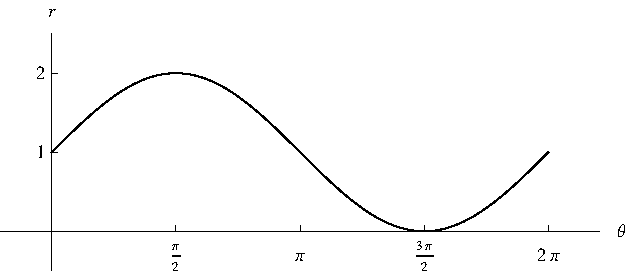
\includegraphics[height=3.6cm]{polar-curves/pictures/11-03-ex7helpera.pdf}%
%}%
%\only<handout:0| 2>{%
%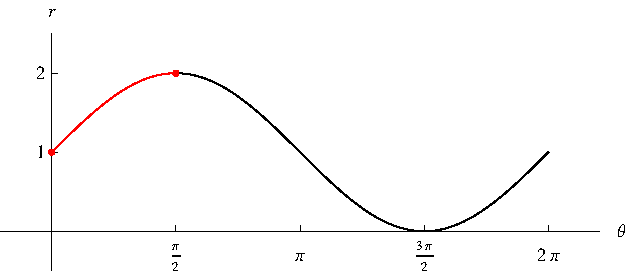
\includegraphics[height=3.6cm]{polar-curves/pictures/11-03-ex7helperb.pdf}%
%}%
%\only<handout:0| 3>{%
%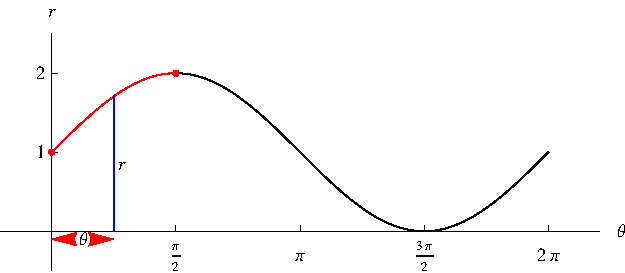
\includegraphics[height=3.6cm]{polar-curves/pictures/11-03-ex7helperba.pdf}%
%}%
%\only<handout:0| 4>{%
%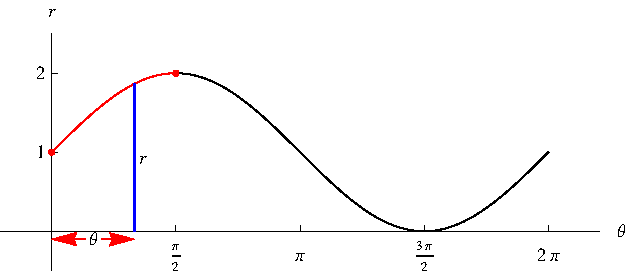
\includegraphics[height=3.6cm]{polar-curves/pictures/11-03-ex7helperbb.pdf}%
%}%
%\only<handout:0| 5>{%
%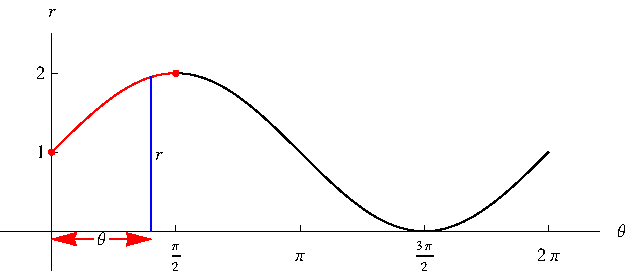
\includegraphics[height=3.6cm]{polar-curves/pictures/11-03-ex7helperbc.pdf}%
%}%
%\only<handout:0| 6>{%
%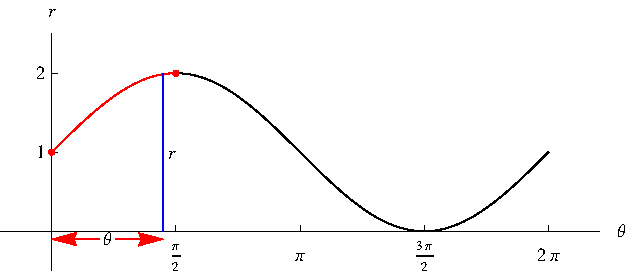
\includegraphics[height=3.6cm]{polar-curves/pictures/11-03-ex7helperbd.pdf}%
%}%
%\only<handout:0| 7>{%
%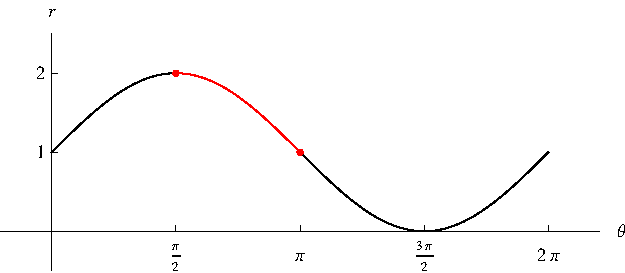
\includegraphics[height=3.6cm]{polar-curves/pictures/11-03-ex7helperc.pdf}%
%}%
%\only<handout:0| 8>{%
%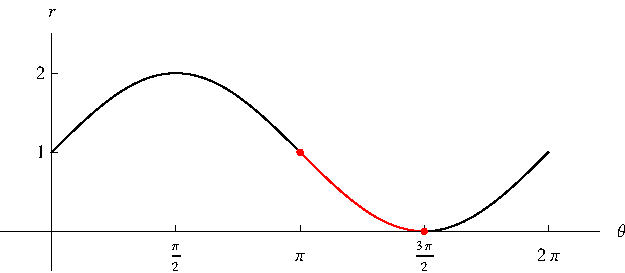
\includegraphics[height=3.6cm]{polar-curves/pictures/11-03-ex7helperd.pdf}%
%}%
%\only<9->{%
%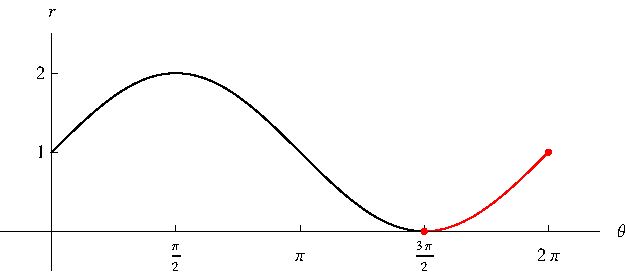
\includegraphics[height=3.6cm]{polar-curves/pictures/11-03-ex7helpere.pdf}%
%}%
\end{columns}
\uncover<1-10>{}
\end{example}
\end{frame}
% end module cardioid-ex7
